\section{Experimental Results}
\label{sec:results}

All micro-F1 values reported in this section use the group-level metric defined in
Section~\ref{sec:task}: a gold group is satisfied by any one of its member codes,
and over-predicting within a group counts as false positives.

\subsection{Individual Component Performance}

Figure~\ref{fig:compbar} shows standalone group-level micro-F1 on our internal test split for each component.
Greek BERT is the strongest single model (0.8196 on the internal test split), ahead of XLM-RoBERTa Base (0.8050).
Dictionary and NER+EL perform comparably; the IR module has the lowest F1 but the
highest recall (0.83), making it a key coverage contributor in the ensemble.

\begin{figure}[htbp]
\centering
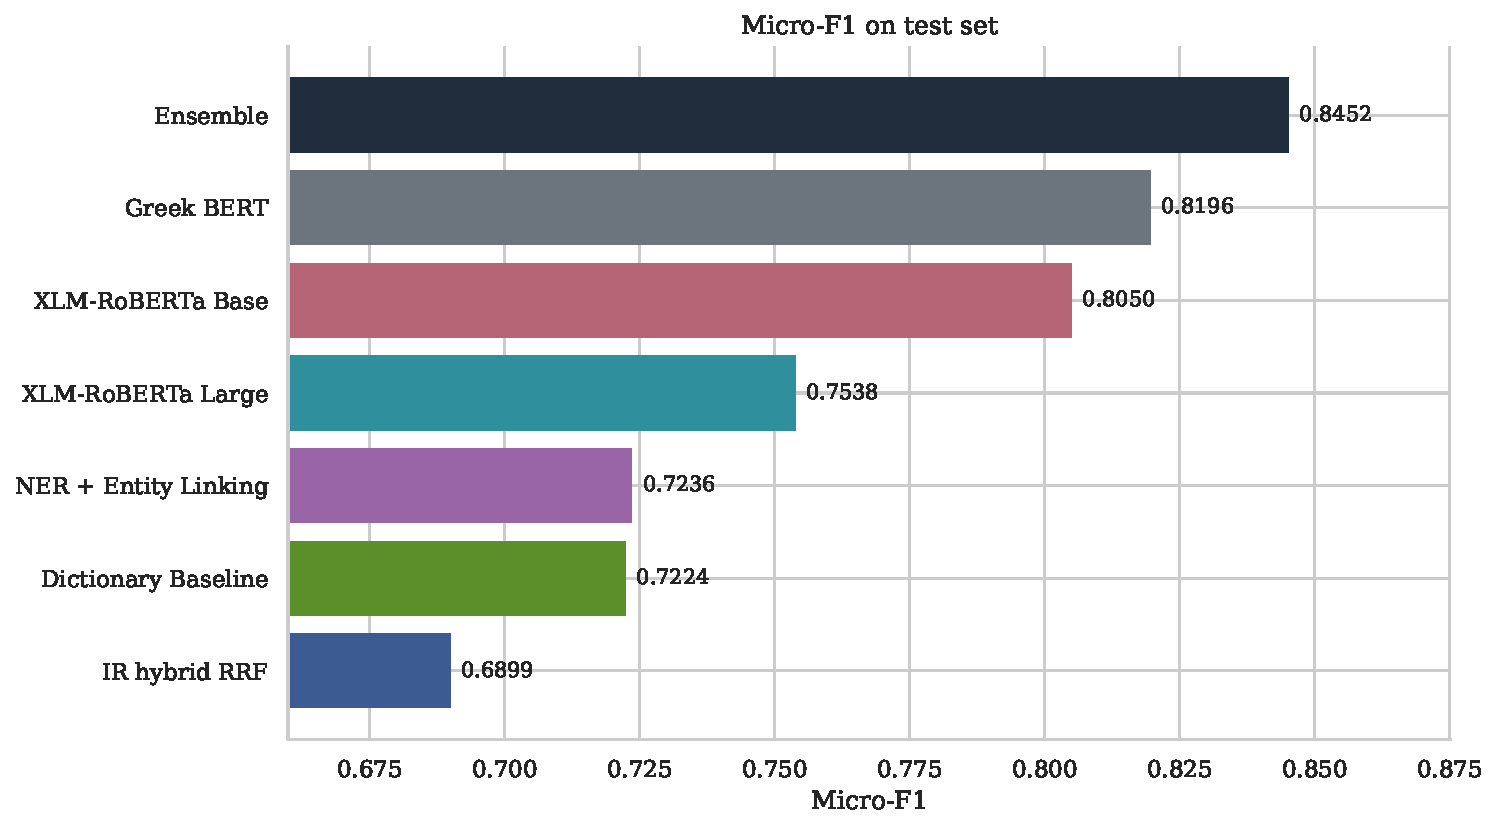
\includegraphics[width=\linewidth]{figures/fig_validation_micro_f1_by_component_bar.pdf}
\caption{Standalone group-level micro-F1 per component on our internal 250-document test split. XLM-RoBERTa Large reports validation F1 (no separate test submission). Official test set scores appear in Table~\ref{tab:results}.}
\label{fig:compbar}
\end{figure}

\subsection{Ablation Studies}

\subsubsection{Threshold tuning.}
Table~\ref{tab:thr} shows the effect of progressively finer thresholding.
Per-label tuning adds $\approx$3.7 percentage points over a fixed $t{=}0.5$ baseline and
$\approx$0.7 percentage points over the global optimum.

\begin{table}[h]
\centering
\caption{Threshold tuning ablation for Greek BERT.}
\label{tab:thr}
\begin{tabular}{lc}
\toprule
Strategy & Val.\ micro-F1 \\
\midrule
Fixed $t=0.5$ & 0.7693 \\
Fixed $t=0.6$ (active) & 0.7984 \\
Global sweep $[0.45, 0.75]$ & 0.7989 \\
Per-label sweep (2-pass) & 0.8062 \\
\bottomrule
\end{tabular}
\end{table}

\subsubsection{Impact of LLRD.}
Layer-wise learning rate decay (factor 0.90) preserves pre-trained lower-layer
representations while adapting upper layers to the clinical domain, most notably
benefiting rare labels.

\subsubsection{Loss function comparison.}
ASL outperformed both binary cross-entropy and focal loss through better recall on rare
labels. BCE gave good precision but lower recall; focal loss improved recall over BCE
but less than ASL due to its symmetric treatment of positive and negative examples.

\subsubsection{Ensemble composition.}
Table~\ref{tab:comp} compares the composition operators. The intersection (merge\_and)
achieves the best F1 by combining the weighted ensemble with the label correction
module's precision boost.

\begin{table}[h]
\centering
\caption{Ensemble composition operator comparison (validation set).}
\label{tab:comp}
\begin{tabular}{lccc}
\toprule
Strategy & Recall & Precision & F1 trend \\
\midrule
Union (merge\_or)         & highest & lowest  & moderate \\
Weighted ensemble         & mid     & mid     & strong \\
$k$-of-$n$ (merge\_k2)   & mid     & mid+    & strong \\
Intersection (merge\_and) & mid$-$  & highest & best \\
\bottomrule
\end{tabular}
\end{table}

\subsection{Official Test Set Results}

Table~\ref{tab:results} reports all five submissions on the official test set. The best
submission uses the merge\_and strategy (weighted ensemble intersected with the label
correction module).

\begin{table}[h]
\centering
\caption{Official ElCardioCC 2026 test set results.}
\label{tab:results}
\begin{tabular}{lccc}
\toprule
Submission & Recall & Precision & F1 \\
\midrule
ensemble (merge\_and: weighted + correction)       & 0.8510 & 0.8830 & \textbf{0.8667} \\
ensemble (merge\_k2: weighted + per-label + corr.) & 0.8687 & 0.8539 & 0.8613 \\
ensemble (safer thr, merge\_k2)                    & 0.8767 & 0.8431 & 0.8596 \\
mlc\_greek\_bert\_100 (100\% data)                 & 0.8194 & 0.8811 & 0.8491 \\
mlc\_greek\_bert (80/10/10 split)                  & 0.8310 & 0.8675 & 0.8489 \\
\bottomrule
\end{tabular}
\end{table}

The ensemble outperforms the best standalone model by +1.8 percentage points (0.8667 vs.\ 0.8491),
confirming the complementarity of the six components. The full-data Greek BERT achieves
virtually the same F1 as the split version (0.8491 vs.\ 0.8489), suggesting the
validation set contributes little additional signal at this scale.

The precision-oriented merge\_and yields the highest overall F1 (0.8667), while
merge\_k2 variants achieve higher recall at the cost of precision, consistent with the
2-of-3 voting design. The safer-threshold merge\_k2 reaches the highest recall (0.8767)
but the lowest precision (0.8431).

\subsubsection{Statistical significance.}
To confirm that the ensemble's gain over the best standalone model is not an artefact
of the small validation set, we compare the weighted ensemble (Table~\ref{tab:weights})
against the best single component (Greek BERT) on the 250-document validation split
using two paired tests. A document-level paired bootstrap (10,000 resamples with
replacement) gives a mean micro-F1 difference of $+0.0323$ (95\% CI $[+0.0212,
+0.0437]$), with zero of the 10,000 resamples favouring the standalone model
($p<10^{-4}$). A McNemar test over gold-group-level outcomes (each gold group counted
as a matched pair: covered by the ensemble only, by Greek BERT only, by both, or by
neither) gives 88 groups recovered only by the ensemble against 21 recovered only by
Greek BERT, a highly significant asymmetry ($p\approx2.6\times10^{-10}$). Both tests
indicate the ensemble's improvement over the strongest individual component is
statistically robust rather than due to chance variation across documents.

\subsection{Computational Complexity}
\label{subsec:complexity}

Table~\ref{tab:complexity} reports backbone parameter counts and observed single-run
wall-clock training time for each component. The neural components dominate training
cost: XLM-RoBERTa Large (560M parameters) takes the longest to converge despite
plateauing at a lower validation F1 (Section~\ref{subsec:xlmr}), while Greek BERT
(113M parameters) reaches its best checkpoint in under 15 minutes over 30 epochs.
The dictionary baseline and information retrieval module involve no gradient-based
training: the former builds its term automaton and applies rule layers in a few
seconds, and the latter's cost is dominated by one-off dense MiniLM encoding of the
document collection, completing in under a minute. At inference time, all components
process the full validation set (250 documents) in well under a minute per
component on commodity hardware (dictionary and IR: single-digit seconds; neural
components: one forward pass per document/chunk), and the metaheuristic ensemble
search itself (10,000 evaluations $\times$ 2 restarts $\times$ 2 optimisers over
precomputed score matrices) completes in under 5 minutes on CPU alone, since it
operates on cached prediction scores rather than raw text.

\begin{table}[h]
\centering
\caption{Backbone parameter counts and single-run training wall-clock time per component.}
\label{tab:complexity}
\begin{tabular}{lrl}
\toprule
Component & Backbone params & Training time \\
\midrule
XLM-RoBERTa Large     & 560M & 2h 14m 52s \\
XLM-RoBERTa Base      & 278M & 1h 35m 43s \\
Greek BERT (mlc)      & 113M & 14m 50s \\
NER+EL (Greek BERT)   & 113M & 3m 05s \\
Information Retrieval & --   & $\approx$30s (no training; one-off dense encoding) \\
Dictionary Baseline   & --   & $\approx$5s (no training; rule construction only) \\
\bottomrule
\end{tabular}
\end{table}

Training times were logged from independent single runs (Weights \& Biases run
duration for the four neural components; direct wall-clock measurement for the
non-neural components) and are not strictly comparable across hardware, but the
order-of-magnitude gap between the neural components and the rule-based/retrieval
components is stable regardless of environment.

\subsection{Error Analysis}

\begin{figure}[htbp]
\centering
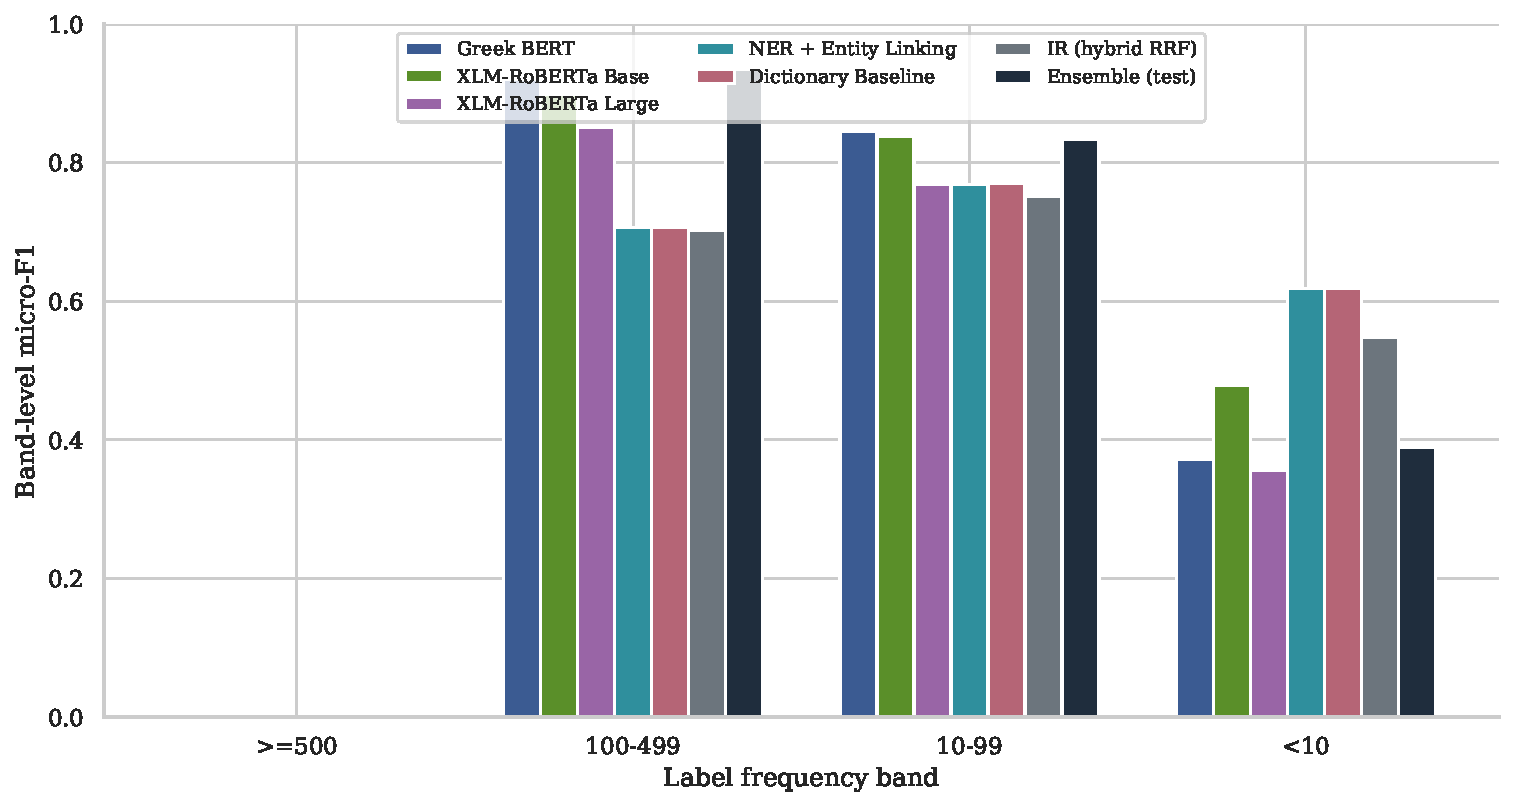
\includegraphics[width=\linewidth]{figures/fig_macro_f1_by_label_frequency_band.pdf}
\caption{Macro-F1 per component across label frequency bands (three bands shown; no code reaches $\geq$500 instances in the 250-document validation set). All models degrade sharply on rare labels ($<$10 instances); the ensemble provides no recovery for this band.}
\label{fig:freqband}
\end{figure}

\begin{figure}[htbp]
\centering
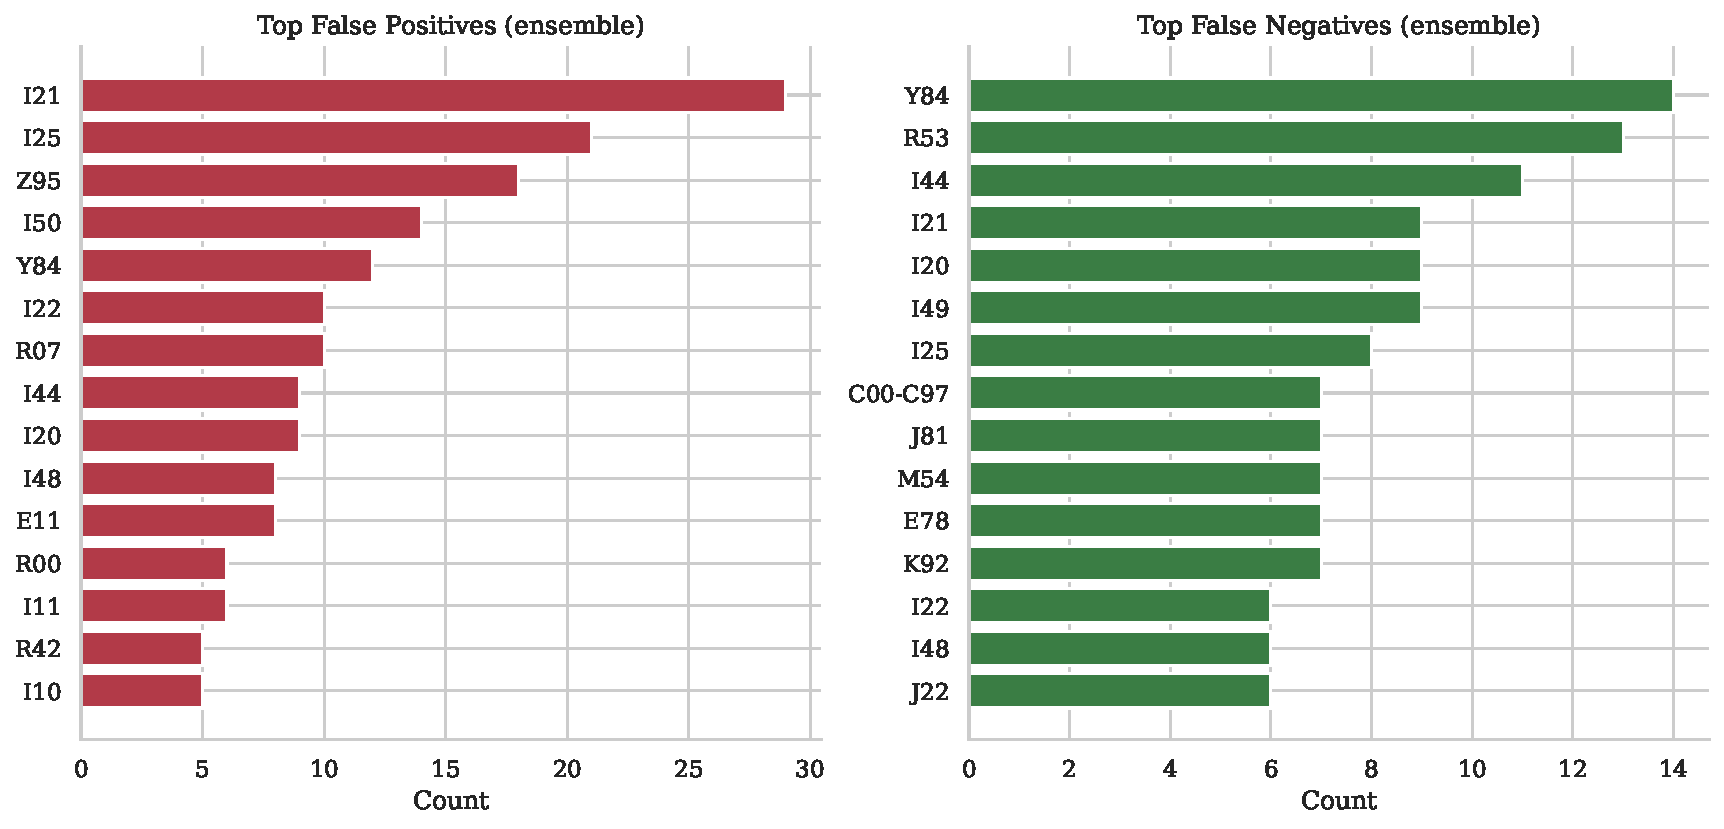
\includegraphics[width=0.85\linewidth]{figures/fig_top_fp_fn_labels.pdf}
\caption{Top false-positive and false-negative codes for the best ensemble submission.}
\label{fig:fpfn}
\end{figure}

\begin{figure}[htbp]
\centering
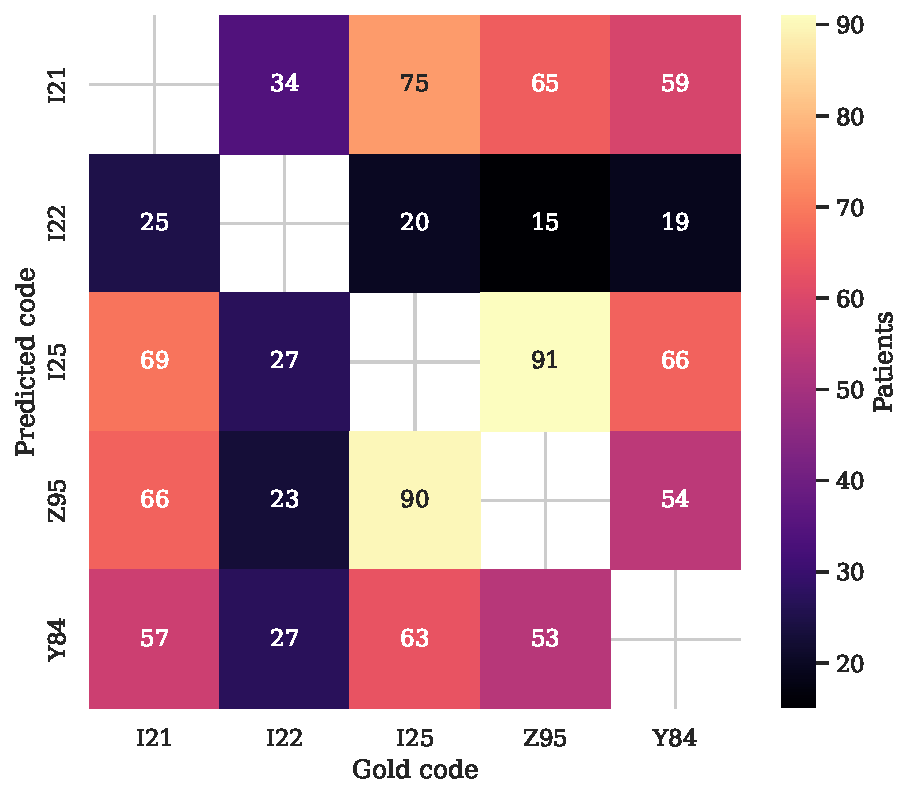
\includegraphics[width=0.65\linewidth]{figures/fig_acute_mi_codes_confusion_cluster.pdf}
\caption{Co-prediction counts for the MI/procedure cluster (I21, I22, I25, Z95, Y84).}
\label{fig:micluster}
\end{figure}

\textbf{Rare labels.} The 30 codes with $<$10 training instances are the primary error source.
For 10 of these, per-label thresholding is not applicable. The dictionary recovers some
(e.g.\ E85 via the amyloidosis rule), but codes with no lexical surface form (e.g.\ M35, R57)
remain unrecovered.

\textbf{Coverage gaps.} 31 label types lie outside the dictionary's coverage, including metabolic
(E00), haematological (D47), and musculoskeletal codes, which require inference from
laboratory values or implicit multi-sentence evidence.

\textbf{Label confusion.} I21/I22/I25 (acute MI, subsequent MI, chronic ischaemic disease) frequently
co-occur and require temporal reasoning to assign correctly, beyond current bag-of-token
models. Z95 (vascular implants) is the main false-positive source due to ubiquitous stent
and pacemaker mentions, motivating the merge\_and correction step.

\textbf{Calibration.} Greek BERT under-predicts rare labels: probabilities for rare codes often fall
below 0.5. Per-label thresholding helps but becomes unreliable for labels with fewer than 15
positive validation examples.
